\documentclass[10pt,a4paper,twocolumn]{article}
\usepackage[margin=18mm,columnsep=6mm]{geometry}
\usepackage[T1]{fontenc}\usepackage[utf8]{inputenc}
\usepackage{mathptmx,microtype,graphicx,amsmath,caption}
\usepackage[numbers,sort&compress]{natbib}\usepackage[hidelinks]{hyperref}\usepackage{xurl}
\setlength{\parindent}{0pt}\setlength{\parskip}{4pt}\setlength{\bibsep}{3pt}
\captionsetup{font=small,labelfont=bf,skip=4pt}
\renewcommand{\dbltopfraction}{.9}\renewcommand{\textfraction}{.05}\renewcommand{\dblfloatpagefraction}{.8}\setcounter{dbltopnumber}{2}
\title{Feeding Frenzy: Who Benefits When Dolphins and Gannets Hunt Together?}
\author{Reuben Stanley\\University of Western Australia}
\date{9 November 2026 | Working draft V3}
\begin{document}\raggedbottom
\twocolumn[\maketitle\begin{center}\begin{minipage}{0.97\textwidth}\textbf{Abstract.} Each winter, South Africa's sardine run brings dolphins, Cape gannets and other predators together around immense schools of fish. Dolphins may drive prey toward the surface, creating feeding opportunities for diving birds. But do gannets also help dolphins, or does adding more hunters simply create competition? We examine these questions in a three-dimensional agent-based model where dolphins use the same local herding-and-striking rule with and without birds. Across four previously examined fish schools, we varied minimum herding duration and gannet number from one to eighteen. Adding birds increased mean dolphin catches in fourteen of eighteen tested combinations. The largest four-school dolphin total was 127 fish versus 91 without birds (+39.6\%), reached with one herding unit and either nine or eighteen gannets. With two herding units and twelve birds, both species gained in all four schools, and dolphins also exceeded their best tested bird-free baseline. Food per gannet generally fell as bird groups grew, even where dolphin presence improved returns against equally sized bird-only groups. The model therefore produces mutual feeding benefits under identifiable conditions, alongside declining per-bird returns. The favourable settings still require independent-school and finer-timestep validation.\par\vspace{8pt}\end{minipage}\end{center}]
\section{Introduction}
The South African sardine run is a spectacular seasonal gathering of fish and predators. As sardines travel along the coast, common dolphins, Cape gannets and other hunters converge on dense schools of prey \citep{teske2021,odonoghue2009}. Dolphins can surround and drive fish toward the surface, where diving birds may find food that would otherwise be difficult to reach \citep{odonoghue2009,licht2026}. From above the water, a feeding frenzy can look like several species working together. But sharing a hunting ground is not the same as both species benefiting.

Access to prey is itself a possible benefit of association. South African sardine habitats extend to about 200 m depth \citep{sanbi2018}, well below the shallow dives recorded for Cape gannets \citep{ropert2004}. Driving prey upward may therefore create access as well as disturb a school. These ecological depths do not define the starting depth or physical scale of our simulations.

Several explanations are plausible. Gannets may largely take advantage of the dolphins' work, arriving after fish have been concentrated near the surface. Alternatively, successive attacks by birds and dolphins may disrupt the school, exposing individual fish to subsequent hunters \citep{lett2014,thiebault2016}. A third possibility is competition: additional predators consume a limited supply of fish or interfere with one another, so that each catches less. These explanations are not mutually exclusive. A bird might gain from dolphin presence compared with an equally large bird-only group, yet receive less food when more birds join the feeding event \citep{licht2026}.

Previous studies support parts of this picture, but leave important comparisons unresolved. During the South African sardine run, gannets have been observed responding to changes in dolphin behaviour \citep{odonoghue2009}. Thiebault and colleagues found that recent predator attacks were associated with improved gannet capture success and modelled how successive attacks disturb fish schools \citep{thiebault2016}; they did not measure matched dolphin feeding returns. In New Zealand, a separate study of common dolphins and Australasian gannets suggested potentially mutual feeding associations, although that is a different field system and species of gannet \citep{stockin2022}. A recent review identifies several ways underwater hunters may help seabirds, while noting that benefits flowing back to underwater hunters remain less certain \citep{licht2026}. We therefore do not claim to be the first to model multiple predators; instead, we use matched simulations to ask who benefits and under what conditions.

Our model follows an already located fish school and compares a fixed dolphin hunting rule with and without gannets. We vary the minimum time dolphins spend herding and the number of birds, then separately measure: (i) whether dolphins catch more when gannets are added, (ii) whether birds catch more when dolphins are present, and (iii) whether food per bird rises or falls as the bird group grows. Figure~\ref{fig:1} introduces the model and an example encounter. These are measures of food captured during a short simulated encounter, not energetic profit, fitness or proof of deliberate cross-species communication.

\begin{figure*}[!t]\centering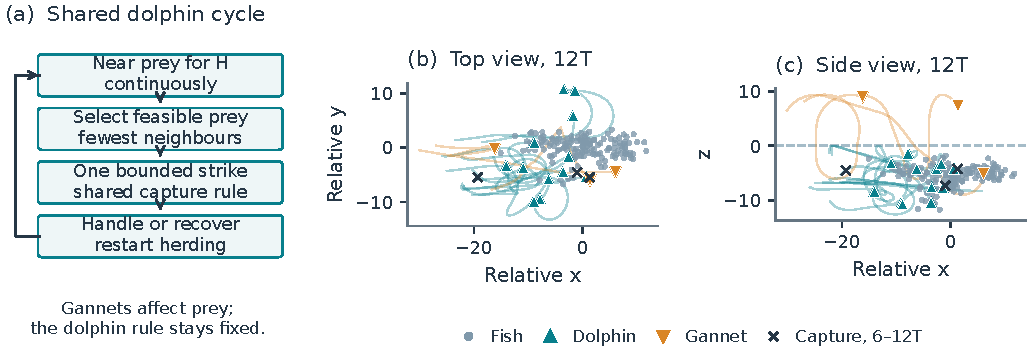
\includegraphics[width=\textwidth]{figures/fig1_model.pdf}\caption{How a model feeding encounter works. (a) Dolphins maintain near-prey pressure for a minimum duration, pursue a feasible target and recover. Their rules do not change with bird presence. (b,c) Top and side views of one recorded encounter at 12 model-time units, with paths and captures from 6--12. This illustrates geometry, not proof of a compact bait ball.}\label{fig:1}\end{figure*}
\section{Model and measurements}
\subsection{Fish dynamics and shared hunting rules}
We simulate 160 schooling fish in three dimensions using the existing C++ FishSim engine and Python predator controllers. Separation, alignment and attraction \citep{couzin2002} occupy disjoint zones bounded by radii 1, 10 and 14; separation takes social priority. With T denoting one model-time unit, fish move at speed 3 model units/T, have a baseline turning limit of \ensuremath{\pi}/2 per T and have zero native movement noise. Migration, depth preference and local escape cues also influence movement. For submerged predators, proximity strength is the maximum across predators: w = max\_j clip(1 - d\_j/4.5, 0, 1). Alignment and attraction weights become 1 - 0.75w and 1 - 0.5w, while predator proximity multiplies the baseline turning limit by 1 + 3w. Birds in flight supply no threat cue. A near-surface downward guard supplements normal steering. The surface is z = 0 and horizontal space is open. All lengths and times are uncalibrated model units; full cue caps and update rules are in the notebook.

Twelve dolphins use exact local prey states within range 25. Each follows waypoints ahead of, beside and below a tracked prey patch. A strike becomes available after continuous proximity within 4.5 units of an observed fish for H = 1, 2 or 3T; lost proximity resets the clock. This is a proxy for sustained herding pressure, not proof of a compact bait ball or coordinated pod roles. After H, a dolphin ranks physically feasible targets within range 6 by fewer fish neighbours inside radius 2, followed by interception and turning time. Dense prey remain eligible and outward motion is not required. A strike lasts at most 6T, with speed 6 and turning limit \ensuremath{\pi}/2 per T. Recovery lasts 2T after capture or 0.75T after failure. Bird presence changes neither this rule nor its capture probability (Figure~\ref{fig:1}).

Gannets use idealised global prey information within detection depth 12. DBSCAN (radius 2; minimum neighbourhood 4) identifies clusters, sampled by accessible fish count before a dense reachable fish is targeted. Birds fly at speed 10, swim at 6 and turn at up to \ensuremath{\pi}/2 per time unit. Flight height is 3, maximum dive depth 12 and bout duration at most 6T. New-target selection reserves turning/ascent space: its depth cap is 12 - 6/(\ensuremath{\pi}/2) - 0.25 \ensuremath{\approx} 7.93 units. A separate travel-feasibility criterion requires estimated travel to the target to fit within the bout's allowed duration. Recovery lasts 2T after capture or 1T after failure and may overlap ascent. With no eligible prey, birds search by flying straight; they do not hold station above a lost school. One bird uses one launch site; groups of three or more use the same three sites with different multiplicity. Predator body-spacing avoidance is absent.

Predators propose motion from the same step-start prey state. Fish advance with submerged-predator cues, swept contacts resolve jointly in time order, and controller memory commits the resolved step. An eligible contact occurs between a point prey and a mouth sphere of radius 0.4, offset forward by 0.3. It succeeds with fixed probability q = 0.7 for both species. The first eligible contact closes the bout whether capture succeeds or fails; a captured fish is removed once. No density-dependent capture or bird-triggered dolphin bonus is imposed.

\subsection{Feeding returns and school measurements}
We measure fish captured per individual. For species s in school i, A(s,i) = C(s,i)/N(s), where C counts uniquely removed prey and N is species abundance. The complete encounter lasts 36T; the rate is A/(36T). Travel, herding, failures and recovery remain in this denominator, even if prey are depleted early. Dolphin comparisons match the same school and herding duration with and without birds; gannet comparisons match the same school and bird count with and without dolphins. Absolute captures per gannet across counts answer the separate group-size question.

Launches count initiated dolphin strikes; eligible contacts count bouts reaching the mouth-contact rule. Pooled contact yield divides total contacts by total launches across schools, rather than averaging their ratios; late launches may be incomplete. For live fish, c is their arithmetic centroid and r90 the 90th percentile distance from c. Outward motion exceeds 0.3 units/T in the radial direction relative to c and mean live-fish velocity. State summaries use trapezoidal time averages of nonempty saved frames, then equal-school means. Prey removal changes the surviving population used by these measures.

\section{Comparisons and uncertainty}
The exploratory experiment uses four previously examined starting schools. Each tests minimum herding durations H = 1, 2 or 3T with zero, one, three, six, nine, twelve or eighteen gannets, plus matched bird-only groups at positive counts. This gives 108 completed condition--school encounters, including eight exact archived replays: the original 60 encounters and 48 higher-count additions. All last 36T at timestep 0.00125T with one capture-randomness setting. Matched treatments reuse fish starts, predator readiness and private-stream initialisations. Schools differ after a common 20T preparation, including in readiness and random-stream states. Replays and shared controls add no independent schools. Exact IDs and seeds remain in the notebook.

Paired changes are averaged equally across schools. The 95\% pointwise percentile intervals estimate uncertainty in these mean changes by resampling whole four-school records 10,000 times, preserving matching and cross-setting dependence. The intervals do not adjust for selecting settings; with four records, positive observed effects cannot generate an unseen negative school in resampling. Raw effects therefore accompany intervals. The strongest tested dolphin-only duration is selected on the same schools and reselected within each resample: a benchmark for the retained rule, not a confirmed optimum.

Because the controller and discovery schools were previously explored, the map is exploratory. A separate check used eight fresh schools, H = 2T and three birds, each in dolphin-only, bird-only and mixed conditions. Original and halved timesteps (0.00125T and 0.000625T) use the same eight starts: numerical treatments, not sixteen schools. The 97.5\% marginal intervals for the two original-timestep primary species comparisons target approximate 95\% familywise coverage; the discovery map instead has 95\% pointwise intervals. Small-sample percentile coverage remains uncertain.

Departure diagnostics cover the original 48 bird-bearing encounters at one, three and six gannets: 36 mixed and 12 bird-only, a subset of the expanded map. Terminal whole-flock contact loss requires every bird to finish in search mode with no eligible new target; a final 6T without launches alone is insufficient. Launches, water entry and the end of committed plunge/pursuit are distinct times. Equal 6T before/after windows require both complete histories; unfinished attacks are right-censored. These are descriptive trajectory comparisons, not new encounters or a causal cessation experiment.

\section{Results}
\subsection{Partner benefits and food per bird}
Figure~\ref{fig:2} separates two meanings of a feeding benefit. Its upper panels show how many fish each dolphin or gannet actually catches; its lower panels show the extra food gained or lost relative to a matched single-species group. Across the eighteen mixed settings, adding birds improves mean dolphin returns in fourteen, leaves one unchanged and reduces three. Gannets gain from dolphin presence in fourteen settings, show no mean change in two and lose in two. These counts describe the tested combinations, not a probability that wild predators benefit.

\begin{figure*}[!t]\centering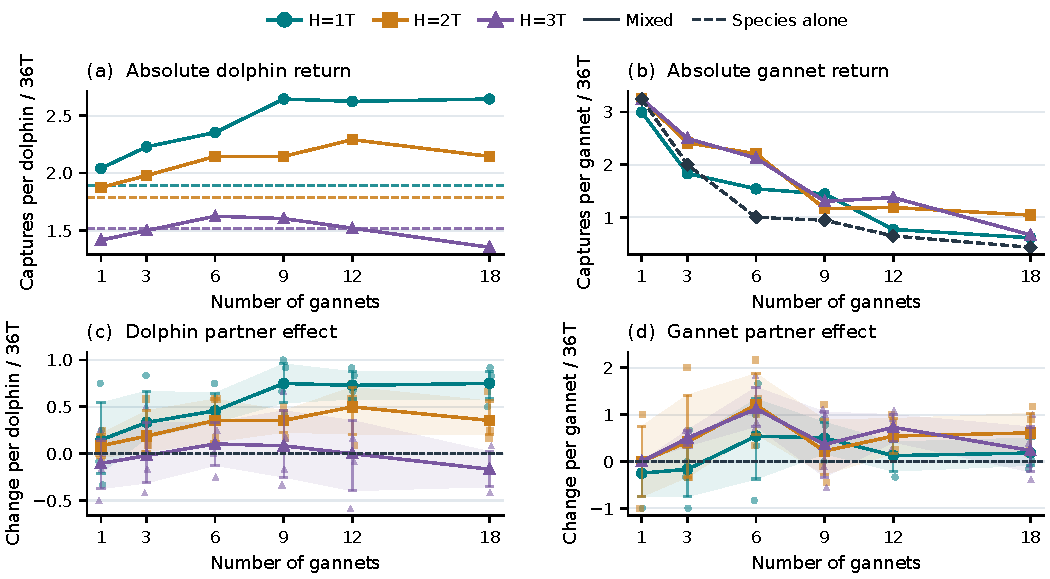
\includegraphics[width=\textwidth]{figures/fig2_returns.pdf}\caption{Absolute feeding returns and matched partner benefits through eighteen gannets. (a,b) Captures per dolphin or gannet over the complete 36T encounter; dashed lines show matched single-species controls. Bird-only controls at each count are shared across H. (c,d) Changes relative to those controls: faint points show four paired school effects; bands and bars are exploratory pointwise 95\% intervals for their means. Actual numeric bird-count spacing is retained.}\label{fig:2}\end{figure*}
Larger gannet groups generally receive less food per bird, although the trend is not monotonic. At H = 2T, mean mixed returns are 3.25, 2.42, 2.21, 1.17, 1.19 and 1.04 fish per bird at one, three, six, nine, twelve and eighteen birds. Same-count bird-only returns are 3.25, 2.00, 1.00, 0.94, 0.65 and 0.43. Thus eighteen birds gain +0.61 fish each from dolphin presence while receiving less than one bird does alone. At every H, per-bird returns are lower at eighteen than at one. This group-size comparison does not isolate competition from changes in access, disturbance or total predator abundance.

The largest observed four-school dolphin total occurs with one unit of minimum herding and either nine or eighteen gannets: 127 captures versus 91 without birds (+39.6\%). We highlight nine birds as the smaller group reaching this maximum, without claiming an optimum. Dolphins gain in all four schools (+8, +12, +5 and +11 fish); the mean is +0.750 fish per dolphin, with a pointwise 95\% interval of [0.542, 0.958]. The corresponding four-school bird total increases from 34 captures alone to 52 with dolphins (+52.9\%): three schools gain and one ties (+8, 0, +7 and +3), giving +0.500 per bird [0.167, 0.833]. These intervals describe settings selected from the same four-school map.

Two herding units and twelve gannets produce mutual gains in all four schools (Figure~\ref{fig:4}a,b). Four-school totals are 110 dolphin captures versus 86 without birds (+27.9\%), and 57 gannet captures versus 31 without dolphins (+83.9\%). Mean gains are +0.500 fish per dolphin [0.208, 0.708] and +0.542 per gannet [0.167, 0.917]. Dolphins also exceed the strongest tested dolphin-only duration, H = 1T: 110 versus 91 captures (+20.9\%). This comparison remains positive in every school (+6, +8, +3 and +2 fish), with a mean +0.396 per dolphin [0.208, 0.583]. Mutual benefit here therefore extends beyond beating only the same-H bird-free control.

\subsection{Herding duration and contact opportunities}
Longer herding changes how often dolphins try to catch fish and how often those attempts reach prey (Figure~\ref{fig:3}a,b). With twelve gannets, the four schools produce 283 dolphin attacks at one herding unit, 218 at two and 166 at three. Contact yield is 0.608, 0.688 and 0.620, respectively. Without birds, the corresponding counts are 251, 197 and 168 launches, with contact fractions of 0.518, 0.614 and 0.595. In both comparisons, H = 2T and 3T yield fewer launches and higher contact fractions than H = 1T. Changing herding time also changes fish trajectories, so these observations do not isolate the cause of better prey access.

\begin{figure*}[!t]\centering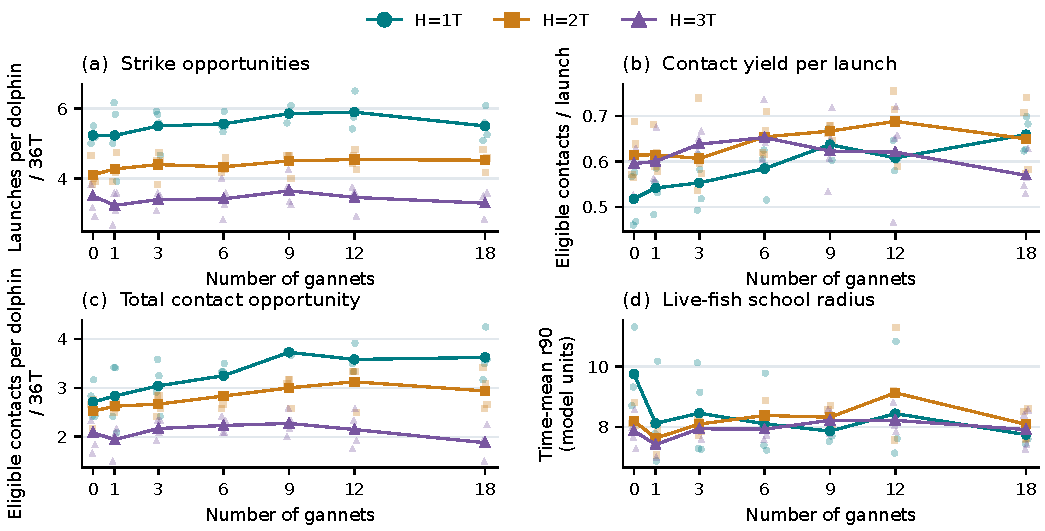
\includegraphics[width=\textwidth]{figures/fig3_opportunities.pdf}\caption{Herding duration changes strike opportunities and prey state. (a) Launches per dolphin; (b) eligible contacts per launch; (c) eligible contacts per dolphin; (d) live-fish r90. Counts cover 36T, including bird-free controls. Faint points show schools; lines join equal-school means except (b), which pools contacts/launches. r90 uses trapezoidal time averages over nonempty frames. School-state changes do not by themselves establish a feeding mechanism.}\label{fig:3}\end{figure*}
At H = 1T with nine birds, bird presence accompanies 12.0\% more dolphin launches, 23.0\% greater contact yield and 37.7\% more contacts (130\ensuremath{\rightarrow}179; Figure~\ref{fig:3}c). Captures rise 39.6\% with contact success fixed at 0.7. These realised changes show more hunting opportunities without a bird-triggered capture bonus. Whole-school radius (Figure~\ref{fig:3}d) does not consistently increase alongside catches; local exposure can change without global expansion, but its contribution has not been isolated.

The response is not a steady rise with bird number. At H = 1T, dolphin captures across the six positive bird counts are 98, 107, 113, 127, 126 and 127. At H = 3T they are 68, 72, 78, 77, 73 and 65, against 73 without birds. Eighteen birds therefore accompany an 11.0\% dolphin loss under the longest herding rule. The largest dolphin and gannet returns occur at different settings: H1/nine birds gives 127 dolphin and 52 bird captures; H2/eighteen birds gives 103 and 75. Nearly equal combined catches conceal different food shares.

\begin{figure*}[!t]\centering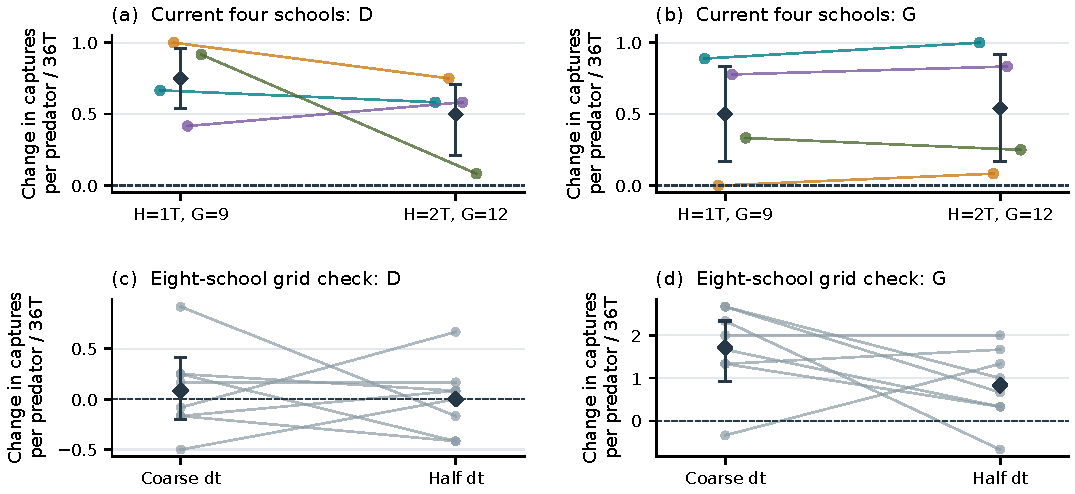
\includegraphics[width=\textwidth]{figures/fig4_sensitivity.pdf}\caption{Selected mutual benefits and separate numerical sensitivity. (a,b) Four-school dolphin and bird effects at H = 1T with nine birds and H = 2T with twelve birds, using matched controls and pointwise 95\% intervals. (c,d) The distinct eight-school H = 2T, three-bird check across original and halved timesteps; only original means have 97.5\% marginal intervals. Axes show changes per individual predator over 36T: twelve dolphins throughout, nine/twelve birds above and three below. Thin lines connect the same school, diamonds mark means, and bars show the stated intervals. Schools and settings must not be pooled.}\label{fig:4}\end{figure*}
\subsection{Depth access and loss of flock contact}
Within the older one/three/six-bird subset, whole-flock contact loss occurred in one of 36 mixed and one of 12 bird-only encounters. Launch pauses were often temporary: 20 of these 48 encounters resumed launching after gaps of at least 6T. In the two contact-loss cases, prey temporarily descended beyond new-target eligibility. During straight-flight search, bird--prey separation increased; when prey became depth-eligible again, targets still failed the travel-feasibility criterion, and hunting did not resume before the encounter ended. In the illustrated mixed case, dolphins finished with 27 captures versus 23 without birds, with no sustained collapse following bird cessation. These observations motivate separate tests of prey depth and bird search, but do not establish a general post-cessation effect.

\section{Discussion and conclusion}
The model produces mutual feeding benefits under identifiable hunting conditions. With H = 2T and twelve gannets, both species gain in all four schools, and dolphins also outperform their best tested dolphin-only duration. Shorter herding produces the largest dolphin return. Partner benefits can coexist with generally declining per-bird food as bird groups grow: the benefit of dolphin presence and the effect of adding birds answer different questions. Reporting only combined catches would conceal these species and individual differences.

Surface herding offers a plausible access benefit for birds \citep{odonoghue2009,thiebault2016,licht2026}, alongside prey disturbance and competition. Other agent-based work reports non-additive predation effects from non-coordinating predators \citep{mohapatra2025}. The departure examples illustrate temporary depth exclusion interacting with the implemented bird search/reacquisition rule; they do not measure how much dolphin herding maintains shallow prey. The present dolphin controller reacts neither to bird number nor dive events. Mutual gains therefore arise without an explicit rule for cross-species coordination.

Limits include fixed uncalibrated contact success, exact local dolphin prey states, idealised global bird information, point fish and absent predator spacing. Captures exclude energy costs, satiety and fitness \citep{thiebault2016,licht2026,stockin2022}. In a separate eight-school H = 2T, three-bird check, halving the timestep changes the mean dolphin gain from +1 fish per school to zero (Figure~\ref{fig:4}c,d); the favourable nine- and twelve-bird settings still need finer-grid and independent-school validation.

The next study should vary both dolphin and gannet numbers while retaining matched single-species controls and reporting captures per individual. Fixed-total-predator comparisons and prey-access measurements would help separate competition from facilitation. Relating attack timing and overlap to feeding returns could identify useful patterns; controlled timing interventions would then test whether synchronisation improves hunting. The present results establish conditional mutual feeding benefits in the model and provide clear settings for those larger tests.

\subsection{Software and reproducibility}
Fish movement inherits \url{https://github.com/yangyushi/FishSim}; predator controllers, completed data and main.ipynb are at \url{https://github.com/reuben-trade/FishSim-Dolphin-Gannet-Pilot}. Default Run All verifies frozen inputs, recomputes counts, means and paired effects through eighteen gannets, redraws Figures 2--4 and loads the archived Figure~\ref{fig:1}. Interval endpoints and time-averaged school-state summaries are retained rather than regenerated from raw trajectories. The notebook labels the separate eight-school grid check and older 48-encounter departure subset, and prints its Python/package versions. Optional model execution is a separate documented workflow; the eight-school replication runner and sweep configuration are distinguished. Exact school IDs, seeds and detailed departure timecourses accompany the notebook.

\begin{thebibliography}{10}
\bibitem{teske2021} Teske PR et al. The sardine run in southeastern Africa is a mass migration into an ecological trap. Science Advances. 2021;7:eabf4514. doi:10.1126/sciadv.abf4514.
\bibitem{odonoghue2009} O'Donoghue SH. The sardine run: investigating sardine and predator distribution in relation to environmental conditions using GIS and remotely sensed products. PhD thesis, University of KwaZulu-Natal; 2009.
\bibitem{lett2014} Lett C, Semeria M, Thiebault A, Tremblay Y. Effects of successive predator attacks on prey aggregations. Theoretical Ecology. 2014;7:239--252. doi:10.1007/s12080-014-0213-0.
\bibitem{thiebault2016} Thiebault A, Semeria M, Lett C, Tremblay Y. How to capture fish in a school? Effect of successive predator attacks on seabird feeding success. Journal of Animal Ecology. 2016;85:157--167. doi:10.1111/1365-2656.12455.
\bibitem{couzin2002} Couzin ID, Krause J, James R, Ruxton GD, Franks NR. Collective memory and spatial sorting in animal groups. Journal of Theoretical Biology. 2002;218:1--11. doi:10.1006/jtbi.2002.3065.
\bibitem{ropert2004} Ropert-Coudert Y, Grémillet D, Ryan P, Kato A, Naito Y, Le Maho Y. Between air and water: the plunge dive of the Cape Gannet Morus capensis. Ibis. 2004;146:281--290. doi:10.1111/j.1474-919x.2003.00250.x.
\bibitem{mohapatra2025} Mohapatra S, Sinha Mahapatra P. Behavioural response of prey to repeated attacks by non-coordinating predators. Scientific Reports. 2025;15:22977. doi:10.1038/s41598-025-05946-6.
\bibitem{licht2026} Licht M, Correia E, Wikelski M, Krause J. How volant seabirds benefit from sub-surface predators during multi-predator feeding aggregations. Philosophical Transactions of the Royal Society B. 2026;381:20250199. doi:10.1098/rstb.2025.0199.
\bibitem{stockin2022} Stockin KA, Amiot C, Meynier L, Purvin C, Machovsky-Capuska GE. Understanding common dolphin and Australasian gannet feeding associations from nutritional and ethological perspectives. ICES Journal of Marine Science. 2022;79(7):2032--2042. doi:10.1093/icesjms/fsac133.
\bibitem{sanbi2018} South African National Biodiversity Institute. South African sardine. 20 May 2018. Accessed 9 November 2026. \url{https://www.sanbi.org/animal-of-the-week/south-african-sardine/}
\end{thebibliography}
\end{document}
